%
% Chapter 3 - Results
%
\chapter{Results}

This chapter shows what has been achieved and developed to this date.\\

As previously written in the project's roadmap and in the last progress report, this project has already a
HTTP server and an Android application that have most of the features that were planned by this date.

\section{Relational database}

As a result of multiples redesigns, here is the database's conceptual model.

\begin{figure}[H]    
    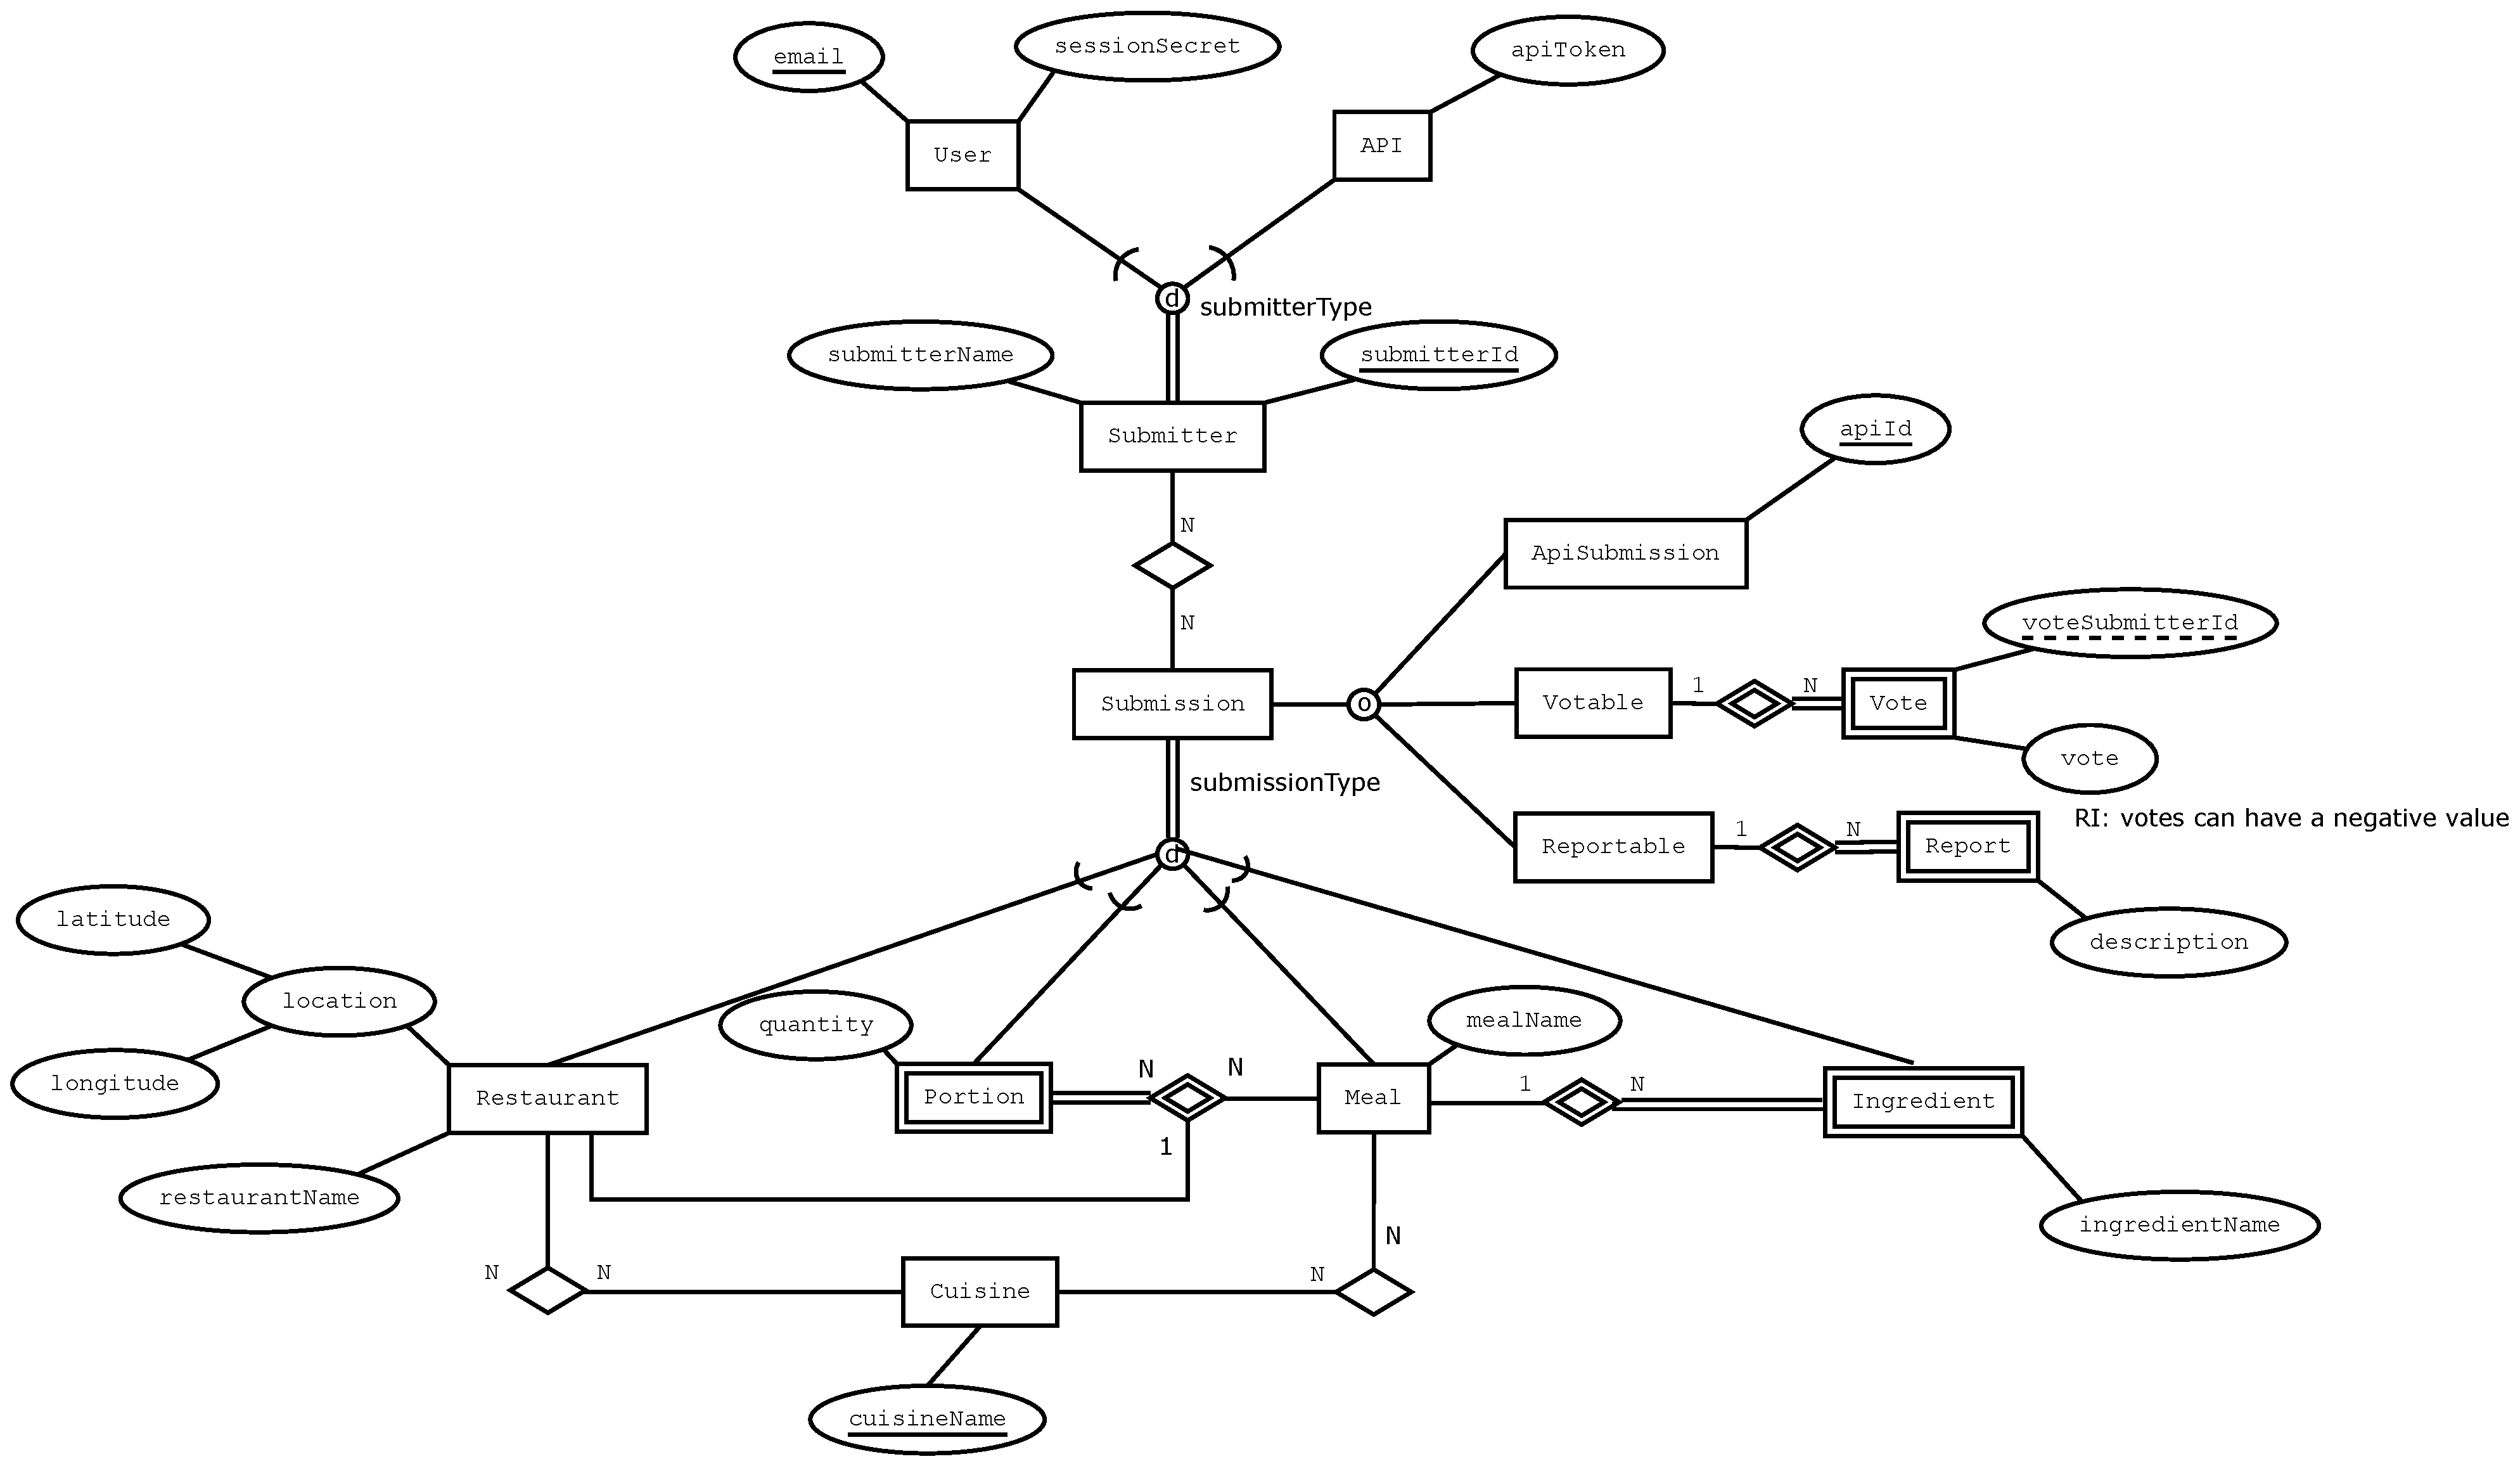
\includegraphics[scale=0.2]{_figures/Nutr.io_Database_Diagram.eps}
    \caption{Database conceptual model}
\end{figure}

\newpage
The database's relational model is present inside this report's appendix [\nameref{app:relational_model}].\\

In the relational model there are tables which are not specified in the conceptual model.
These are a product from associations between entities which will simplify queries' complexity.\\

Now the submission can fall into 4 categories: ApiSubmission, Reportable, Favorable and Votable, in order to disguish between submissions that
are from the user or from APIs and to separate which ones can be reportable, favorable and votable by the user.\\

The cuisine entity has now an associated entity called ApiCuisine, to save cuisine information provided by the Here API.\\

Meals and ingredients were now condensed into one entity called food - now each meal can have meals inside it that can also be considered
ingredients in other contexts.\\

Therefore each meal possesses nutritional information, which is essential to the user especially to the insulin calculations. That information is composed by
'carbs' - meal's carbohydrates; and quantity - meal's quantity.\\

\section{HTTP server}

TODO\\
Some endpoints were changed [\nameref{app:endpoints_table}] in order to meet with the current server requirements.

\section{Geolocation}

Given how all clients rely on obtaining nearby restaurants, there was a need to implement a geolocation function in the project's design.\\

Initial research showcased two possible solutions: Haversine distances and cartesian distances, where the latter returns a highly imprecise distances.
As such, Haversine was selected.\\

The next step was to choose which system filters nearby restaurants: database or HTTP server. After some discussion, the group decided that database was the best
option for two reasons: 
\begin{itemize}
    \item Given the large amount of existing restaurants, sending such data from the database to the HTTP server so that it could filter it would occupy too much memory;
    \item PostgreSQL already supplies extensions that add support for location queries, namely PostGIS.
\end{itemize}

\section{Android application}

As mentioned in the progress report, the group managed to implement in the mobile application a fragment that displays a map with a list of restaurants nearby the user.\\

The user can also search for restaurants, meals and cuisines providing the associated name or identifier.\\

The core feature of the apllication was also finished during this time period - the insulin calculator. This feature calculates how many insulin doses should be injected
in order to maintain the blood glucose levels stabilized according to the user's planned glucose objective for that period of the day.\\

The blood glucose objective is set inside the user's profile, by creating multiples insulin profiles, each one has a limited time period to give the user freedom to map its
own insulin routine throughout the day.\\

This is due to the fact that user's insulin sensitivity factor varies along the day, so the user has the ability to specify its own values in order to the calculator

\\TODO - add fragments